\chapter*{Appendix B:\\Calculations of Spin Density in DiTS}

\begin{figure}[h]
\center
	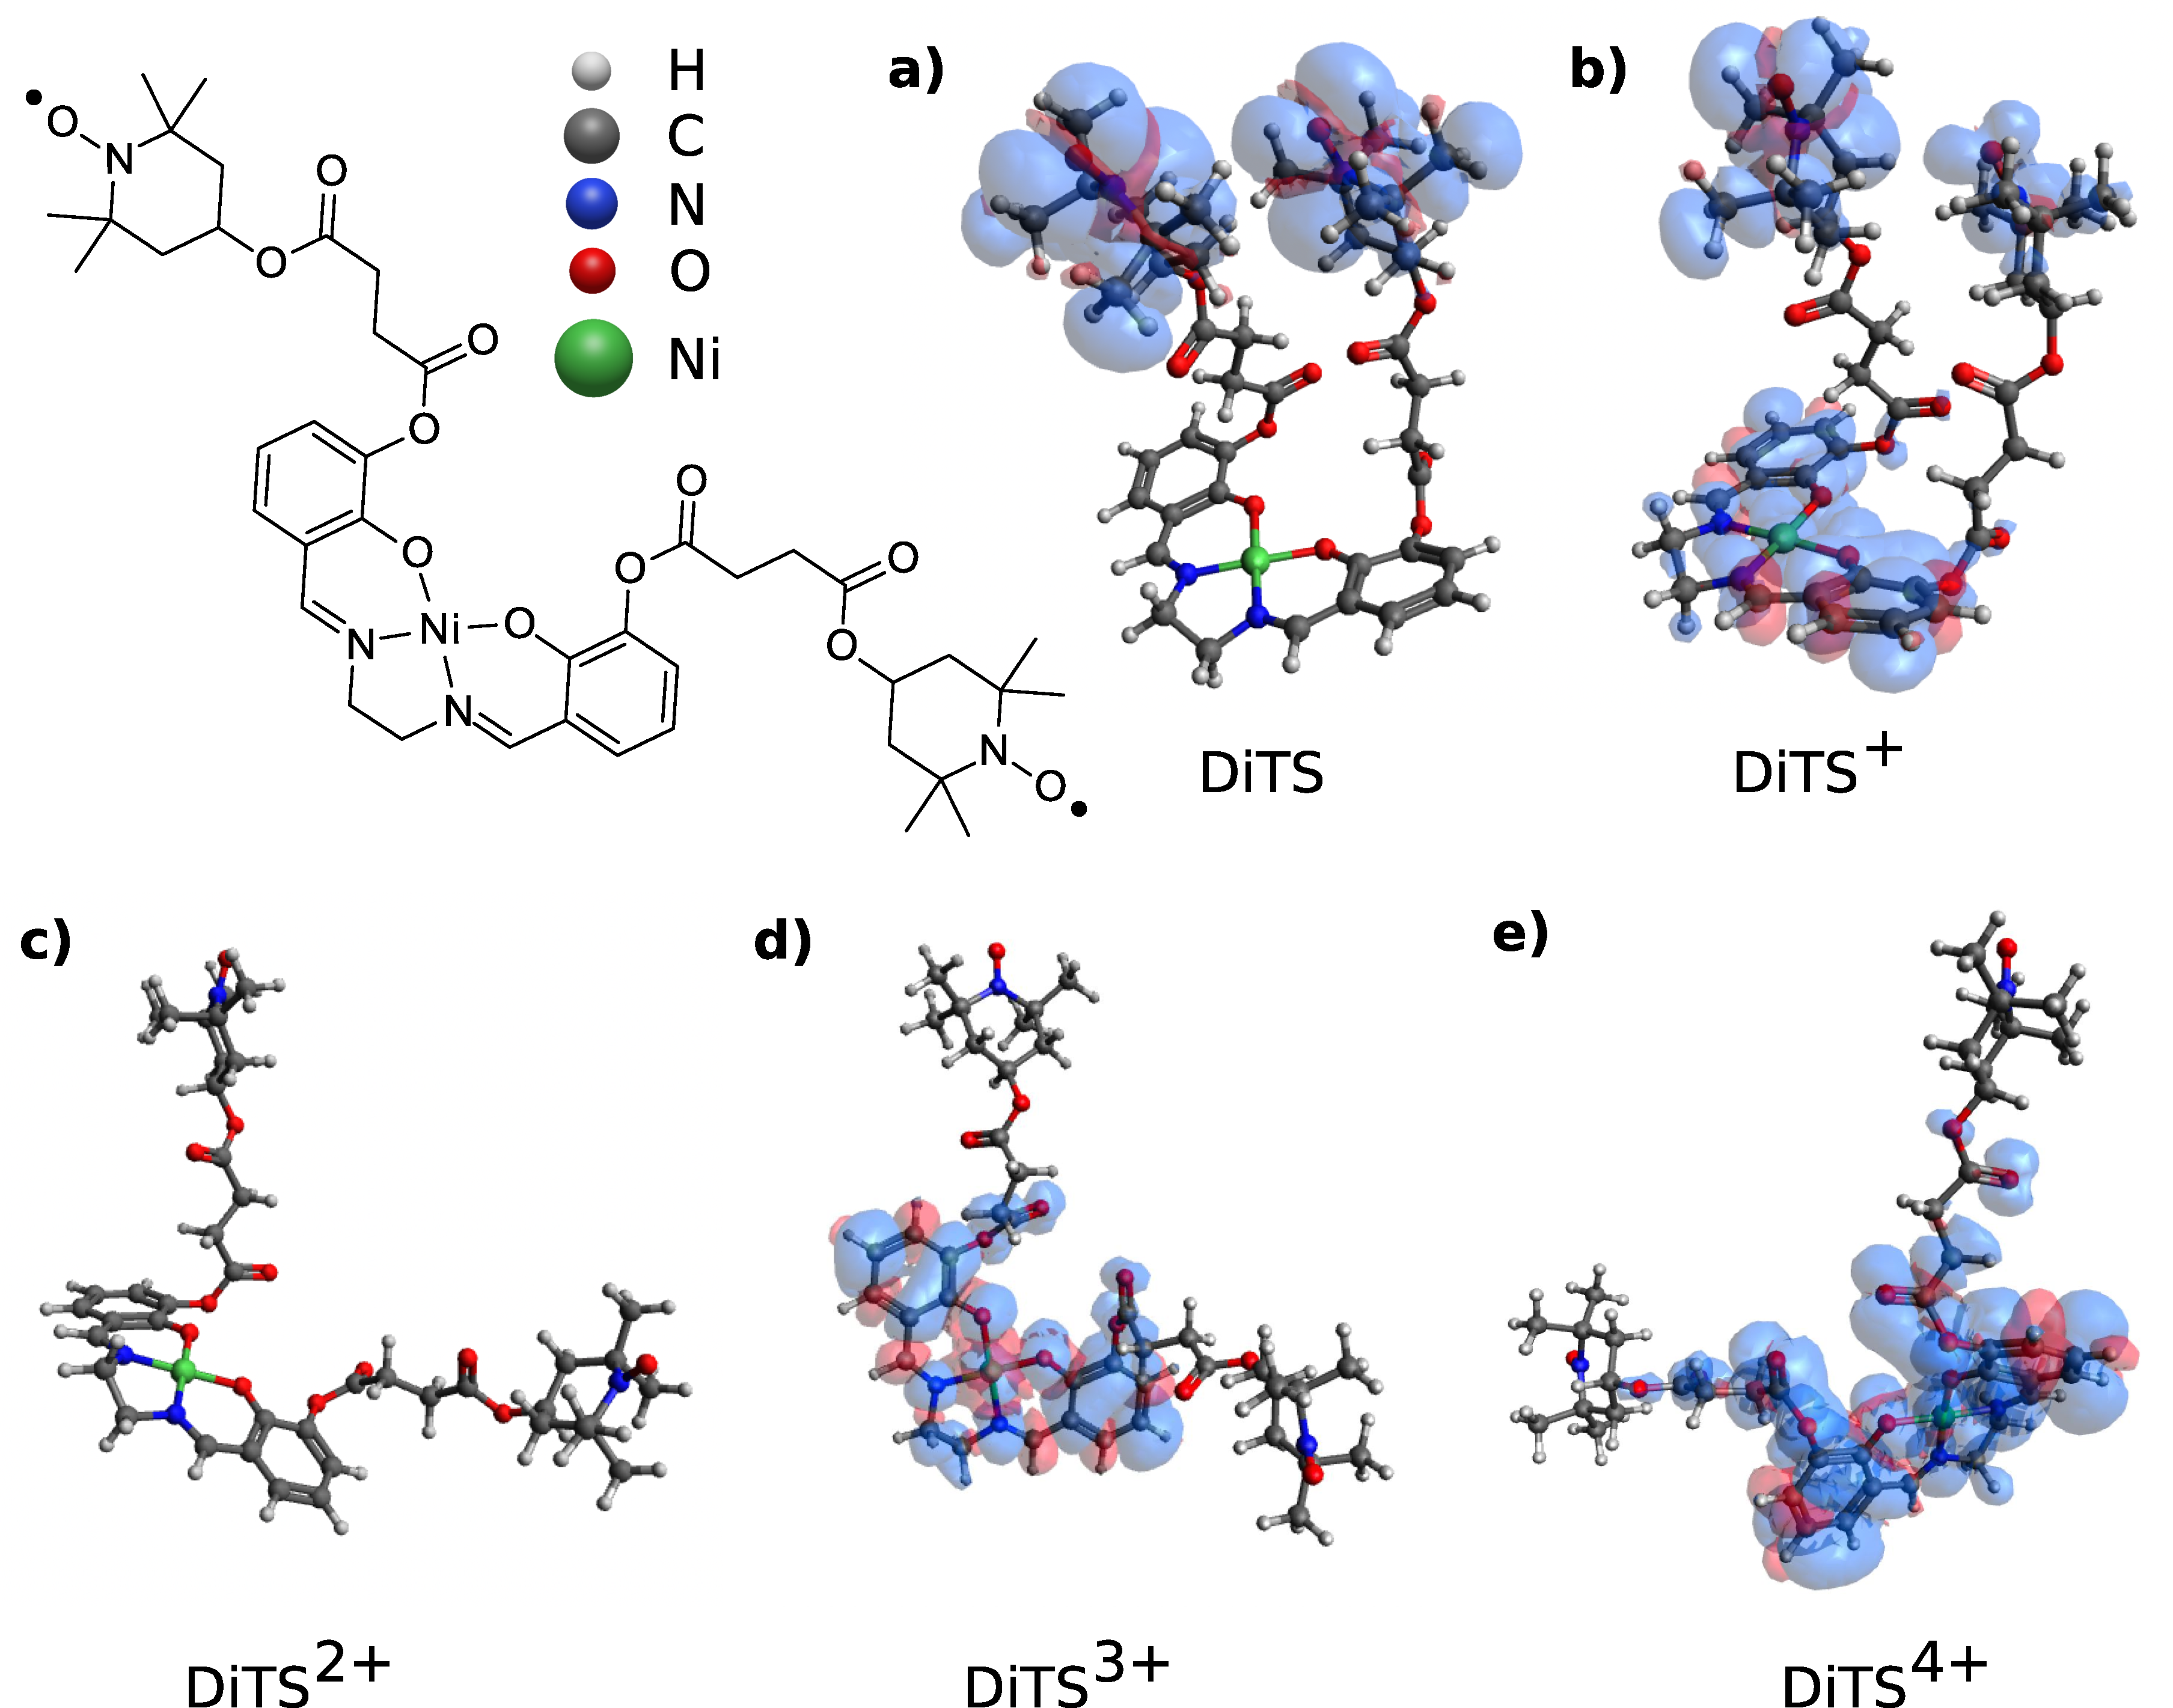
\includegraphics[width=1\textwidth]{./electrochemistry/figures/DFT_DITS.pdf}
	\caption{Spin density in a single DiTS monomer unit for various oxidation states (isovalue: 0.01) calculated with density-functional theory in ORCA~\cite{ORCA}, using the def2-TZVP functional basis set for the geometry optimization and the calculations of the spin density. The calculations were carried out at the high-performance computing cluster Curta of the Free University of Berlin~\cite{Curta}. a): neutral DiTS with two TEMPO radicals, b) singly oxidized DiTS (one hole injected), b) doubly oxidized DiTS showing no spin density, c) DiTS$^{3+}$ showing a positive polaron localized on the NiSalen backbone, d) DiTS$^{4+}$ showing increased spin density on the backbone. Calculations performed by Marcel Gauglitz.}
	\label{fig:DiTS_DFT}
\end{figure}

